\begin{surferPage}[216奇异点]{带有更多实奇异点的曲面}
如前所述,7次曲面上具体的最大奇异点数$\mu(7)$是不知道的。我们仅仅有一个下界和上界:$99\le \mu(7) \le 104$。对一般的次数$d$的曲面我们知之甚少。至少,索尼娅布雷斯科, 奥利弗莱布斯以及范斯滕森利用了奇穆托夫的一个构造使得当今最大奇异点数也能够在带实奇异点的曲面上实现。
至今,我们知道如下结果\[0,41\bar{6}d^3 \lessapprox \mu(d) \lessapprox 0.44\bar{4} d^3.\]
从上可知,我们可以看到此构造的对称性以及与黑胞腔极大数目间的关系。
 \begin{center}
      \begin{tabular}{c@{\qquad}c}
        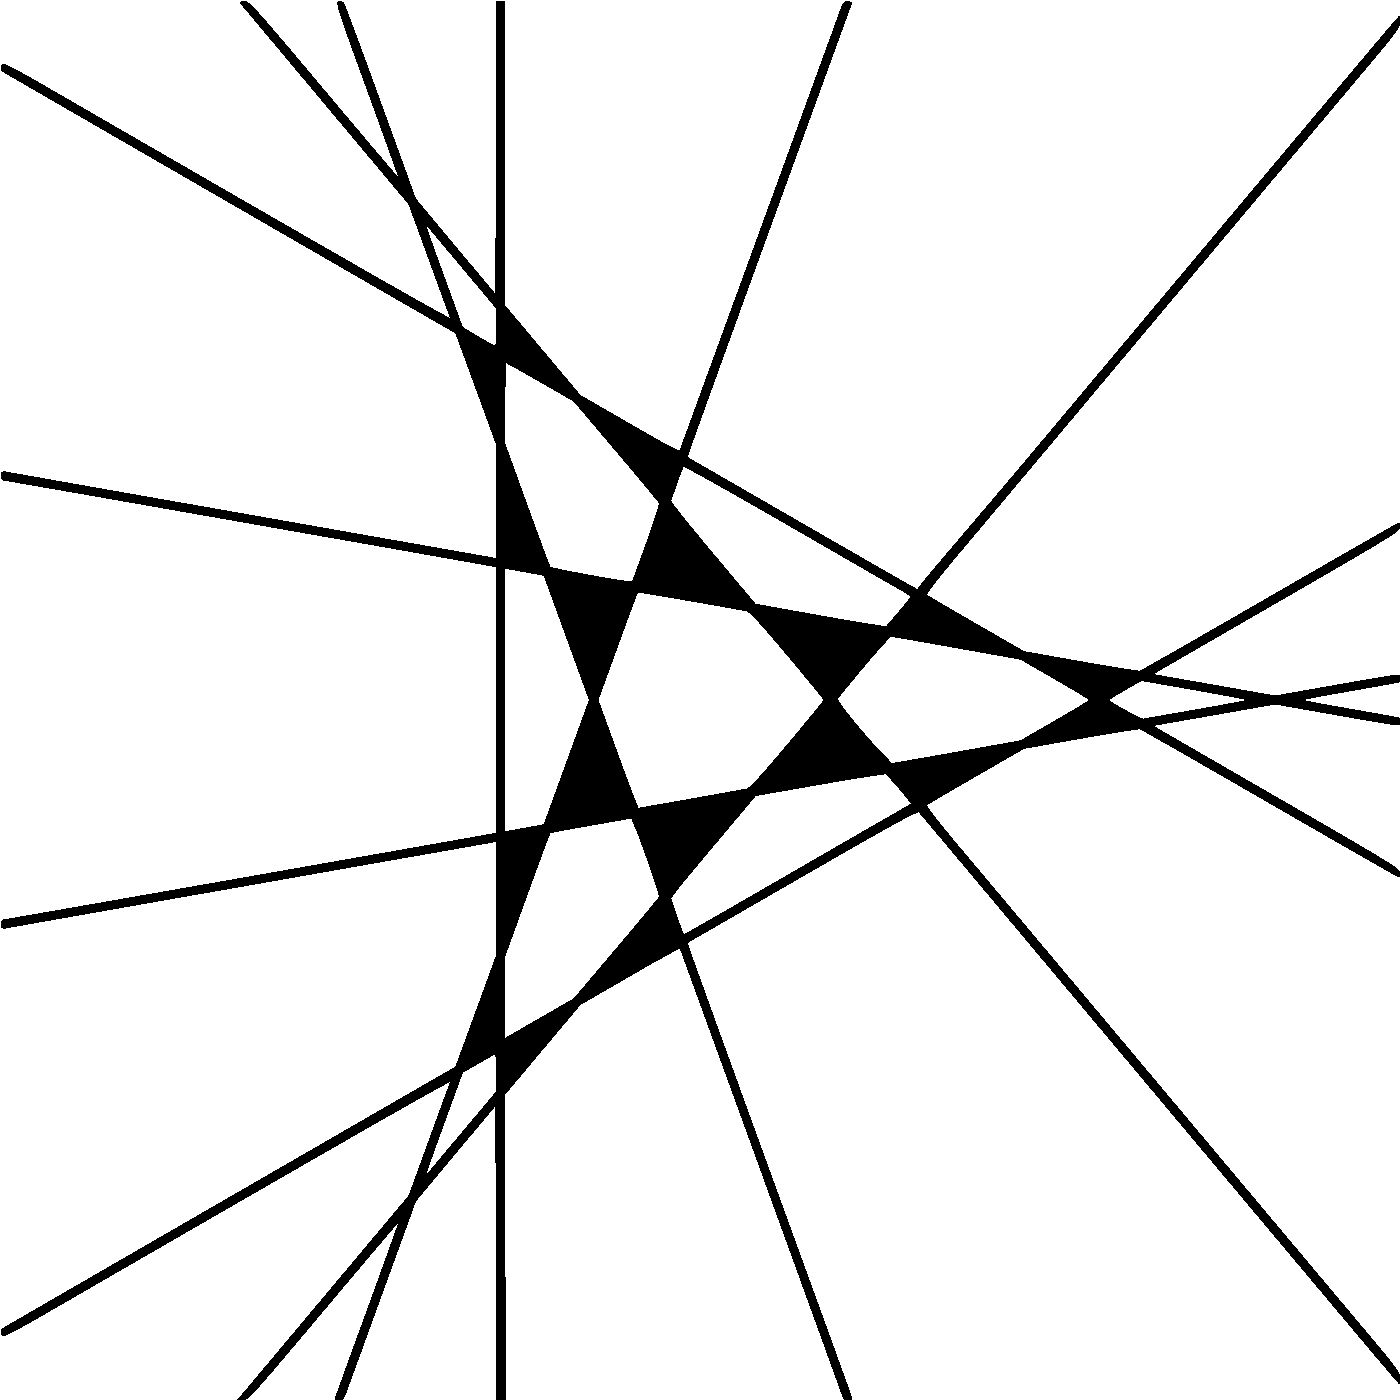
\includegraphics[height=1.5cm]{./../../common/images/vielesing.pdf}
        &
        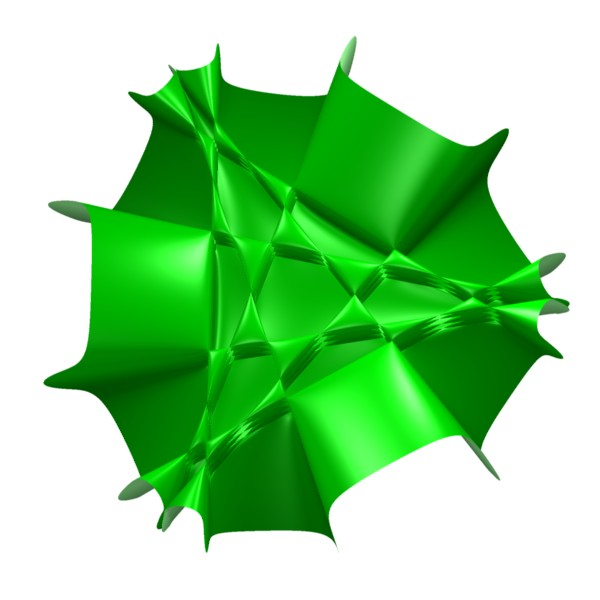
\includegraphics[height=1.5cm]{./../../common/images/p9surface_von_oben}
      \end{tabular}
    \end{center}
\end{surferPage}
